\section{Données nécessaires}
\paragraph{}
Comme il a été mentionné précédemment, les données sont extrêmement importantes.
Nous avons besoin qu'elles soient variées, dans des scénarios différents, c'est-à-dire des arrière-plans différents, des poses de tête différentes, etc.
% As it was mentioned earlier, data is extremely important.
% We need it to be varied, in different scenarios, meaning different backgrounds, different head poses and so on.

\paragraph{}
Nous travaillerons avec des images de la webcam et nous nous concentrerons uniquement sur le visage de l'utilisateur.
Nous en extrairons les yeux et nous travaillerons avec ceux de la première phase.
Ensuite, nous étudierons comment utiliser davantage d'informations, comme la pose de la tête, etc.
Pour chaque expérience, nous mentionnerons les données que nous utiliserons et la manière dont elles ont été traitées.
% We will work with images from the webcam and we will focus solely on the user's face.
% From that, we will extract the eyes and work with those in the first phase.
% Afterwards, we will look into how we can use more information, like the head pose and so on.
% For every experiment, we will mention the data we will be using and how that data has been processed.

% ========== Data Collection Section ==========
\section{Acquisition de données}

\subsection{Moyens d'acquérir des données}
\paragraph{}
Pour la collecte des données, j'ai mis en place deux méthodes: une méthode ``active'' et une méthode ``de fond''.
Pour la méthode active, l'utilisateur doit suivre des yeux le curseur lorsqu'il se déplace sur l'écran.
Chaque fois que le curseur se déplace, une image est capturée de l'utilisateur qui regarde le curseur.
% For collecting data, I have implemented 2 methods: an ``active'' method and a ``background'' one.
% For the active method, the user has to follow with his eyes the cursor as it moves around the screen.
% Every time the cursor moves, an image is captured of the user looking at the cursor.
\paragraph{}
La méthode ``de fond' signifie que l'utilisateur peut utiliser l'ordinateur comme il le souhaite, mais les données seront recueillies pendant ce temps.
Chaque fois qu'il cliquera quelque part, une image sera capturée et enregistrée avec la position de la souris.
% The ``background'' method means that the user may use the computer however he likes, but data will be gathered in this time.
% Every time he will click somewhere, an image will be captured and saved along with the mouse position.

\begin{lstlisting}[language=Python, caption=Collecte de données]
def start_collecting(self, collection_type="background"):
    print(f'Start collecting data in {collection_type} mode')
    WebcamCapturer.start_capturing()
    self.gui.start()
    print('DataCollectorGUI started')
    if collection_type == "background":
        self.mouse_listener.start_listening()
        print('Mouse listener started')
    else:
        threading.Thread(target=self.start_active_collection).start()
\end{lstlisting}

\subsection{Sauvegarde des données}
\paragraph{}
Lorsque la collecte des données est terminée, je les enregistre sous forme de ``session''.
Chaque session est définie par le nombre d'images qui ont été capturées, la résolution de l'écran et la résolution de la webcam.
Vous pouvez voir ci-dessous la structure des dossiers et vous pouvez constater que les images ont été sauvegardées sans les modifier.
% When gathering data is done, I save these as a ``session''.
% Each session is defined by the number of images that were captured, the screen resolution and the webcam resolution.
% Below you can see the folder structure and you can see that the images were saved without doing any modifications to them.

\begin{figure}[H]
    \centering
    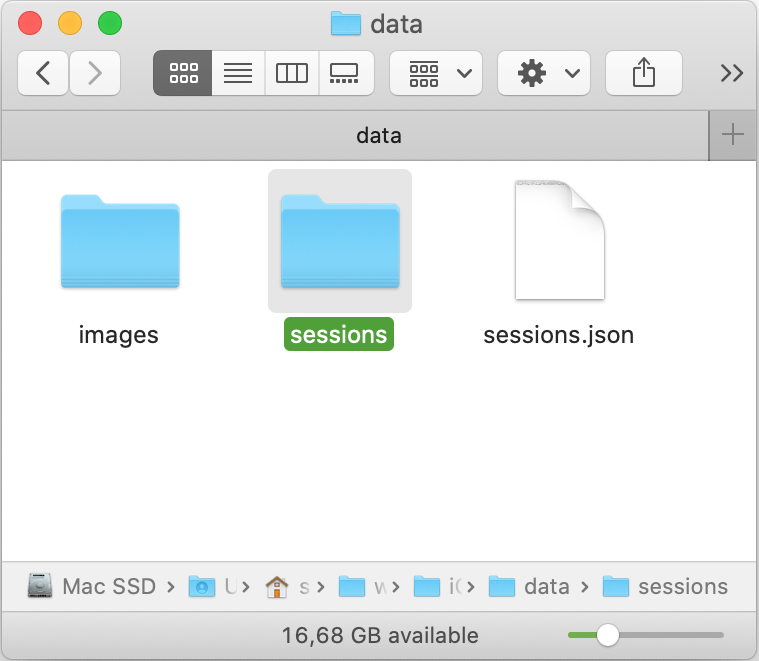
\includegraphics[width=\textwidth/3 - 5pt]{data_structure_1.png}
    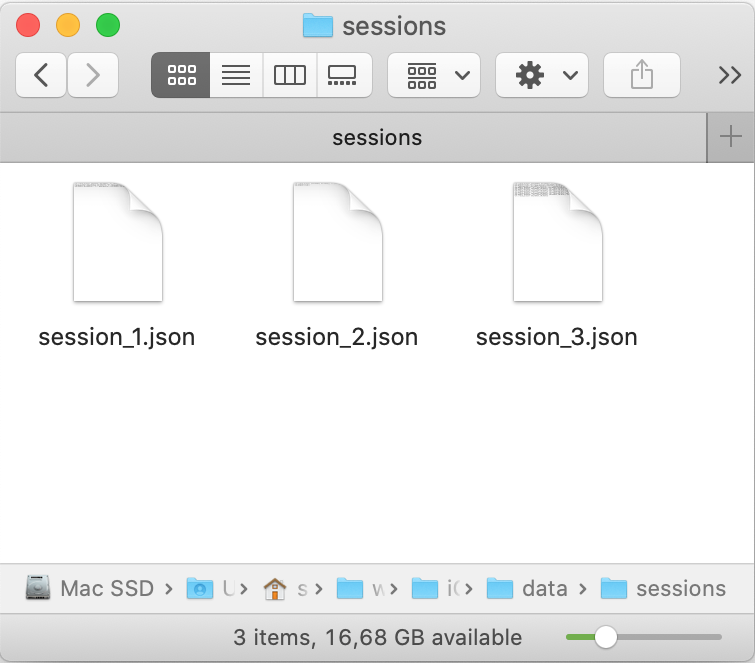
\includegraphics[width=\textwidth/3 - 5pt]{data_structure_2.png}
    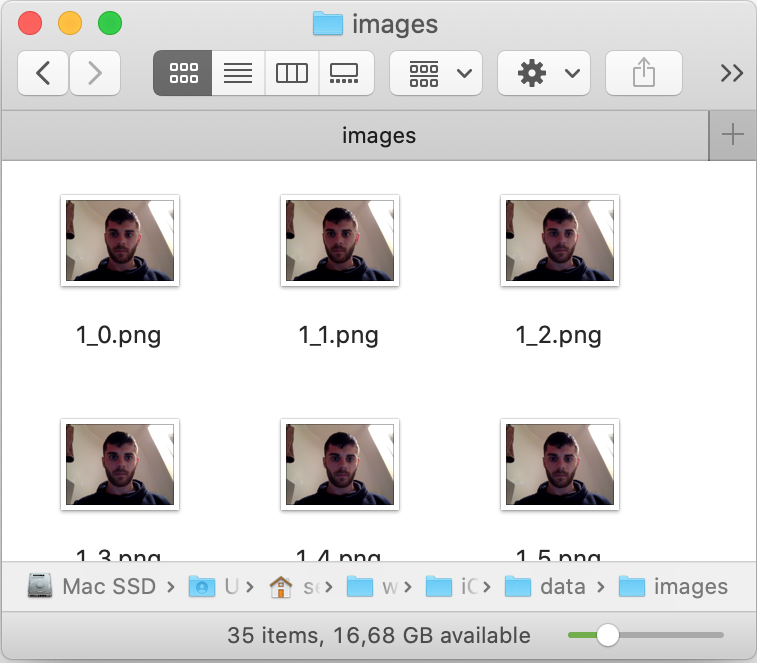
\includegraphics[width=\textwidth/3 - 5pt]{data_structure_3.png}
    \caption{How data is structured}
\end{figure}

\begin{lstlisting}[language=Python, caption=Sauvegarde des données]
def save_collected_data(self):
    if len(self.collected_data) == 0:
        return
    self.collect_data_lock.acquire()
    session_no = self.get_session_number()
    print(f"Saving data for session_{session_no}")
    self.save_session_info(session_no)
    self.save_images_info(session_no)
    self.save_images(session_no)
    self.collect_data_lock.release()
    print('Saving data done')
\end{lstlisting}

% ~~~~~~~~~~ Data Collection Section ~~~~~~~~~~